\chapter{Technol\'ogia}\label{chapter:technologia}
\section{Felhasználói felület}
Az alkalmazás felhasználói felületét a React könyvtár segítségével valósítottam meg.
A React egy nyílt forráskódú JavaScript könyvtár, amelyet a Facebook fejlesztett ki.
A könyvtár célja, hogy a felhasználói felület fejlesztését egyszerűbbé tegye.
A React egy komponens alapú könyvtár, amely lehetővé teszi a fejlesztők számára,
hogy újra felhasználható komponenseket hozzanak létre, amelyeket összeállítva
komplex felhasználói felületeket hozhatnak létre.
\\
\\
\textbf{Komponensek}
A React komponensek egyfajta sablonok, amelyek a felhasználói felület egy részét írják le.
A komponensek egy egyszerű JavaScript objektumok, amelyeknek van egy render metódusa,
amely visszaadja a komponens felhasználói felületét.
\\
\\
\textbf{Komponensek főbb tulajdonságai:}
\begin{itemize}
    \item Paraméterek (props)
    \item Gyerekei (children)
    \item Állapotai (state)
    \item Életciklus metódusai (lifecycle)
    \item Eseménykezelői (event)
    \item Stílusai (style)
    \item Referenciák (ref)
    \item Kontextusai (context)
    \item Típusai (type)
    \item Kulcsai (key)
\end{itemize}
\subsection*{React és Angular összehasonlítása}
A front-end keretrendszer választása fontos lépése az implementáció előkészítésének. Két népszerű keretrendszer képezte a lehetőségek listáját: az Angular és a React.
\\
\\
\textbf{Különbség a React és az Angular között:}
\begin{table}[h]
    \centering
    \begin{tabular}{|l|l|l|}
        \hline
                               & React           & Angular                 \\
        \hline
        Egyszerűség            & Könnyű tanulni. & Több beépített funkció. \\
        \hline
        Flexibilitás           & Rugalmas.       & Kevesebb szabadság.     \\
        \hline
        Teljesítmény           & Virtuális DOM.  & Two-Way Data Binding.   \\
        \hline
        Ökoszisztéma           & Nagy közösség.  & Minőségi eszközök.      \\
        \hline
        Fejlesztői tapasztalat & JSX.            & TypeScript.             \\
        \hline
    \end{tabular}
    \caption[Különbségek React és Angular között]{Különbségek React és Angular között}
\end{table}
\subsection*{Redux vagy Context API}
Az alkalmazás állapotainak kezelésére több lehetőség is felmerült, közöttük a Redux és a Context API.
A Redux egy állapotkezelő könyvtár, amely lehetővé teszi az alkalmazás állapotának tárolását egy központi helyen.
A Context API egy React API, amely lehetővé teszi az alkalmazás állapotának tárolását és megosztását a komponensek között.
Mivel az alkalmazás kis méretű, ezért a Context API-ra esett a választás.
\\
\\
\textbf{A Context API főbb tulajdonságai:}
\begin{itemize}
    \item \textbf{Beépített megoldás:} A Context API része a React alapkönyvtárnak, nincs szükség külső függőségekre.
    \item \textbf{Egyszerűség:} A Context API egyszerűbb és könnyen megérthető, kevesebb boilerplate kóddal.
    \item \textbf{Nincs middleware:} Nem támogat middleware-eket alapból, így aszinkron állapotfrissítéseket manuálisan kell kezelni.
    \item \textbf{Nem optimalizált nagy alkalmazásokhoz:} Nagy alkalmazásokban hatékonytalan lehet, mert minden Context változásra újrarendereli az összes fogyasztót, hacsak nem optimalizáljuk manuálisan.
    \item \textbf{Kevesebb eszköz:} Kevesebb beépített eszköze van, mint a Redux-nak, de ez nem mindig hátrány, függ a projekt igényeitől.
\end{itemize}
\textbf{Példa a Context API állapotkezelésére:}
\begin{lstlisting}[style=es6, morekeywords={document, P5, katex},caption={Context API állapotkezelés}]
    // context
    const CounterContext = React.createContext();
    
    // state and update
    const [count, setCount] = useState(0);
    
    // state refresh
    setCount(count + 1);
\end{lstlisting}

\vspace{2em}

\textbf{A Redux főbb tulajdonságai:}
\begin{itemize}
    \item \textbf{Optimalizáció:} Redux kifejezetten optimalizált a nagyobb alkalmazások számára, és lehetővé teszi az állapot frissítéseinek finom szabályozását.
    \item \textbf{Middleware Támogatás:} Redux lehetőséget ad middleware-ek használatára, amelyek lehetővé teszik az aszinkron állapotfrissítések könnyebb kezelését.
    \item \textbf{Tesztelhetőség:} A Redux architektúrája miatt a tesztelés egyszerűbb, minden action egy független egység, és a reducer funkciók tiszta függvények.
    \item \textbf{Eszközök és Közösség:} Redux-nak nagy közössége van, és sok kiegészítő eszköz, például a Redux DevTools.
    \item \textbf{Boilerplate Kód:} Több boilerplate kód szükséges, hogy elindítsunk egy Redux-alapú állapotkezelést.
\end{itemize}
\textbf{Példa a Redux állapotkezelésére:}
\begin{lstlisting}[style=es6, morekeywords={document, P5, katex},caption={Redux állapotkezelés}]
    // action
    const incrementAction = { type: 'INCREMENT' };
    
    // reducer
    function counterReducer(state = 0, action) {
      if (action.type === 'INCREMENT') {
        return state + 1;
      }
      return state;
    }
    
    // dispatch
    dispatch(incrementAction);
\end{lstlisting}
\vspace{1em}
\subsection*{TypeScript vagy JavaScript}
A TypeScript egy nyílt forráskódú, szigorúan típusos programozási nyelv,
amely a JavaScriptre épül, lehetővé teszi a statikus típusok használatát,
és minden érvényes JavaScript kód érvényes TypeScript kódnak is számít.
Inkább a TypeScript mellett döntöttem, mert a statikus típusok használata
növeli a kód minőségét és a fejlesztési sebességet, illetve csökkenti a hiba lehetőségek számát.

\section{Szerveroldali Logika és API-k}
A szerver és a kliens közötti kommunikáció megvalósításához az ASP.NET Core-t használtam.
Az ASP.NET Core egy nyílt forráskódú, cross-platform, magas teljesítményű keretrendszer,
amelyet a Microsoft fejlesztett ki.
Az ASP.NET Core-t a webalkalmazások és a webes API-k fejlesztésére használják.
A környezetet a C\# programozási nyelvhez tervezték, de támogatja a többi .NET nyelvet is.
Én a megvalósítás során a C\# nyelvet használtam.
Ebben a fejezetben bemutatom a szerveroldali logikát és az API-kat.

\subsection*{Adatbázis}
Az alkalmazásnál MS SQL adatbázist használtam, mert a Microsoft SQL Server-t használom a személyes projekteimhez.
Az MS SQL (Microsoft SQL Server) egy relációs adatbázis-kezelő rendszer (RDBMS) a Microsofttól. Jól skálázható, és számos fejlett funkcióval rendelkezik,
mint például tárolt eljárások,
triggerek és nézetek
. Gyakran használják vállalati szintű alkalmazásokban,
és támogatja a SQL nyelvet az adatok lekérdezésére és manipulálására.
Támogatja az ACID tulajdonságokat és a tranzakciós integritást.
Az ER modell-t használtam az adatbázis tervezéséhez.
Ezt majd a Backend fejlesztési folyamatánál részletezem.

\subsection*{Entity Framework Core}
Az Entity Framework Core (EF Core) egy objektum-relációs leképzési (ORM) keretrendszer a Microsofttól,
amely .NET Core és .NET 5+ alkalmazások számára készült.
Lehetővé teszi a fejlesztők számára, hogy magas szintű,
objektumorientált API-n keresztül dolgozzanak adatbázisokkal,
anélkül hogy közvetlen SQL lekérdezéseket kellene írniuk.
Támogatja a code-first és a database-first megközelítéseket,
így rugalmasságot biztosít az adatmodell és az adatbázisséma kialakításában. Az EF Core lehetővé teszi a LINQ (Language Integrated Query) használatát,
ami természetes módon illeszkedik a C\# és más .NET nyelvekhez.

\begin{figure}[H]
    \centering
    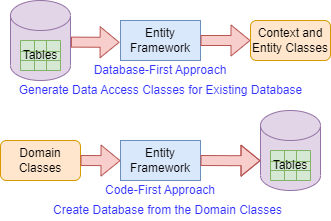
\includegraphics[width=10.0truecm]{images/EntityFramework.png}
    \caption{Entity Framework Core}
    \label{fig:entity_framework_core}
\end{figure}

Skálázható és teljesítmény-optimalizált, ezért alkalmas mind kis,
mind nagyobb vállalati projektekben. Az EF Core támogatja a többszörös adatbázis-motorokat, beleértve az SQL Server, PostgreSQL, SQLite és másokat is.
Az adatmigrációk egyszerű kezelése és automatikus generálása az egyik előnye, ami könnyebbé teszi az adatbázisséma változásainak kezelését.
A keretrendszer beépített támogatással rendelkezik a tranzakciókezelésre, így az ACID tulajdonságok biztosítottak. Az EF Core rugalmas konfigurációs lehetőségekkel rendelkezik,
és jól integrálódik más .NET Core szolgáltatásokkal, mint például a Dependency Injection. Folyamatosan fejlődik és aktívan karbantartott,
így a legújabb .NET technológiákhoz és az adatbázis-technológiákhoz is gyorsan alkalmazkodik.

\subsection*{API}
Az alkalmazásnál RESTful API-t használtam, mert a RESTful API-kat a leggyakrabban használják,
és a legtöbb fejlesztő ismeri őket. A REST (Representational State Transfer) egy architektúrális stílus,
amelyet a webes alkalmazásokhoz használnak. A RESTful API-kat a REST architektúra alapelvei alapján tervezik.
A RESTful API-kat a HTTP protokollra építik, és a HTTP metódusokat használják a kérések kezelésére.
Ennek megvalósításához a \textit{ControllerBase} osztályt használtam a Controllerekben.
Ami teljesen implementálja a RESTful API-kat, és a HTTP metódusokat.

\begin{figure}[H]
    \centering
    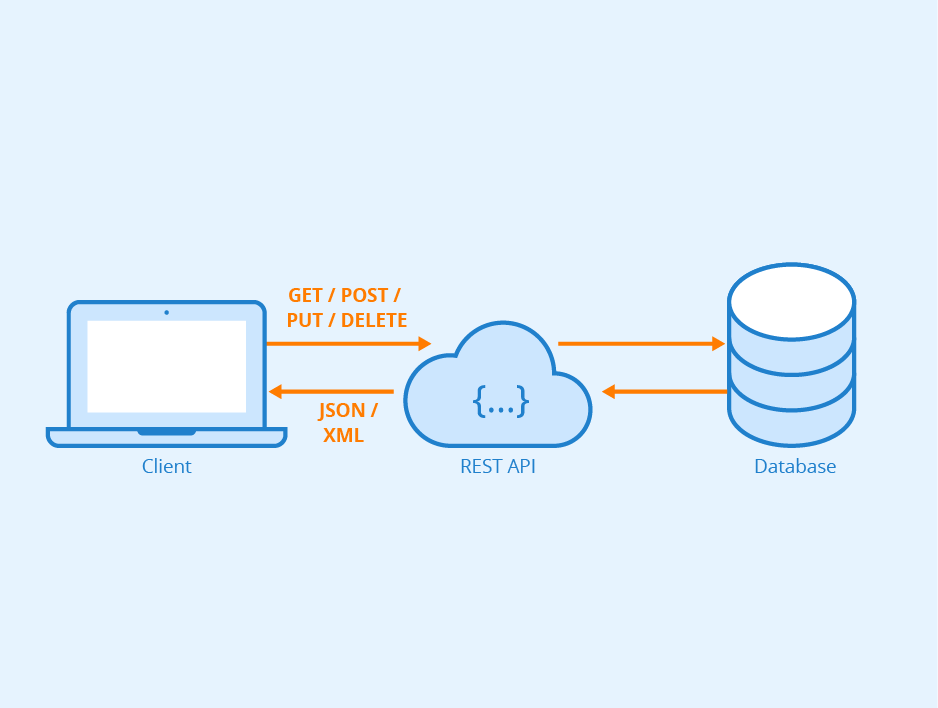
\includegraphics[width=9.0truecm]{images/Rest-API.png}
    \caption[RESTful API]{RESTful API \cite{restfulapi}}
    \label{fig:restfulapi}
\end{figure}

A videók lejátszása során különös figyelmet fordítottam
az állapotkezelésre. Ennek érdekében a WebSocket
protokollt alkalmaztam. A WebSocket egy kétirányú
kapcsolatot tesz lehetővé a böngésző és a szerver között.
Bár a HTTP protokollra épül, mégis képes valós idejű
kommunikációra. A kommunikáció HTTP portokon keresztül zajlik,
ami rugalmasságot ad az alkalmazásnak.
SignalR-t használtam a WebSocket protokoll megvalósításához.

A SignalR egy Microsoft által fejlesztett aszinkron könyvtár,
amely valós idejű webes alkalmazások építését támogatja.
Lehetővé teszi a szerver és a kliensek közötti kétirányú
kommunikációt, gyakran WebSockets használatával.

\begin{figure}[H]
    \centering
    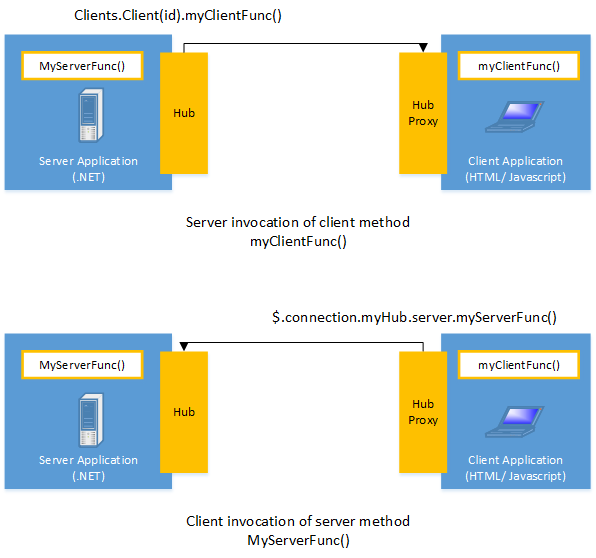
\includegraphics[width=9.0truecm]{images/SignalR.png}
    \caption[SignalR]{SignalR \cite{signalR}}
    \label{fig:signalR}
\end{figure}

Ez eltér a hagyományos HTTP "kérés-válasz" modelltől,
mivel a szerver aktívan küldhet üzeneteket a klienseknek.
Gyakori alkalmazási területei közé tartoznak a chat szolgáltatások,
online játékok és élő adatfrissítések. A SignalR automatikusan választja ki a legmegfelelőbb kommunikációs mechanizmust a szerver és a kliens között,
például long polling, ha WebSockets nem érhető el. A könyvtár könnyen integrálható más .NET technológiákkal és keretrendszerekkel, például ASP.NET Core-al.
A SignalR segítségével könnyen implementálhatók komplex forgatókönyvek, például csoportos üzenetküldés vagy kapcsolatok kezelése. Az állapotkezelés és a kiváló skálázhatóság további előnyei a SignalR használatának.
Mivel a SignalR API az ASP.NET Core része, az infrastruktúrát és a biztonsági mechanizmusokat is könnyen ki lehet terjeszteni rá. Összességében a SignalR egy erőteljes eszköz a valós idejű webes alkalmazások fejlesztéséhez.
\subsection*{Fejlesztői környezet}
Én a Visual Studio 2022-t használtam a fejlesztéshez, mert ez az egyik legnépszerűbb IDE a .NET fejlesztők körében.
A Visual Studio 2022 egy integrált fejlesztői környezet (Integrated Development Environment, IDE), amelyet a Microsoft fejlesztett ki. Ez a platform különösen népszerű a Windows alapú alkalmazások fejlesztésénél, de támogatja számos programozási nyelvet és technológiát, így a fejlesztők széles spektruma számára kínál megoldásokat. Az IDE magába foglalja a kódszerkesztést, a debuggolást, a verziókezelést és más, a fejlesztési ciklusban fontos eszközöket is.
\begin{figure}[H]
    \centering
    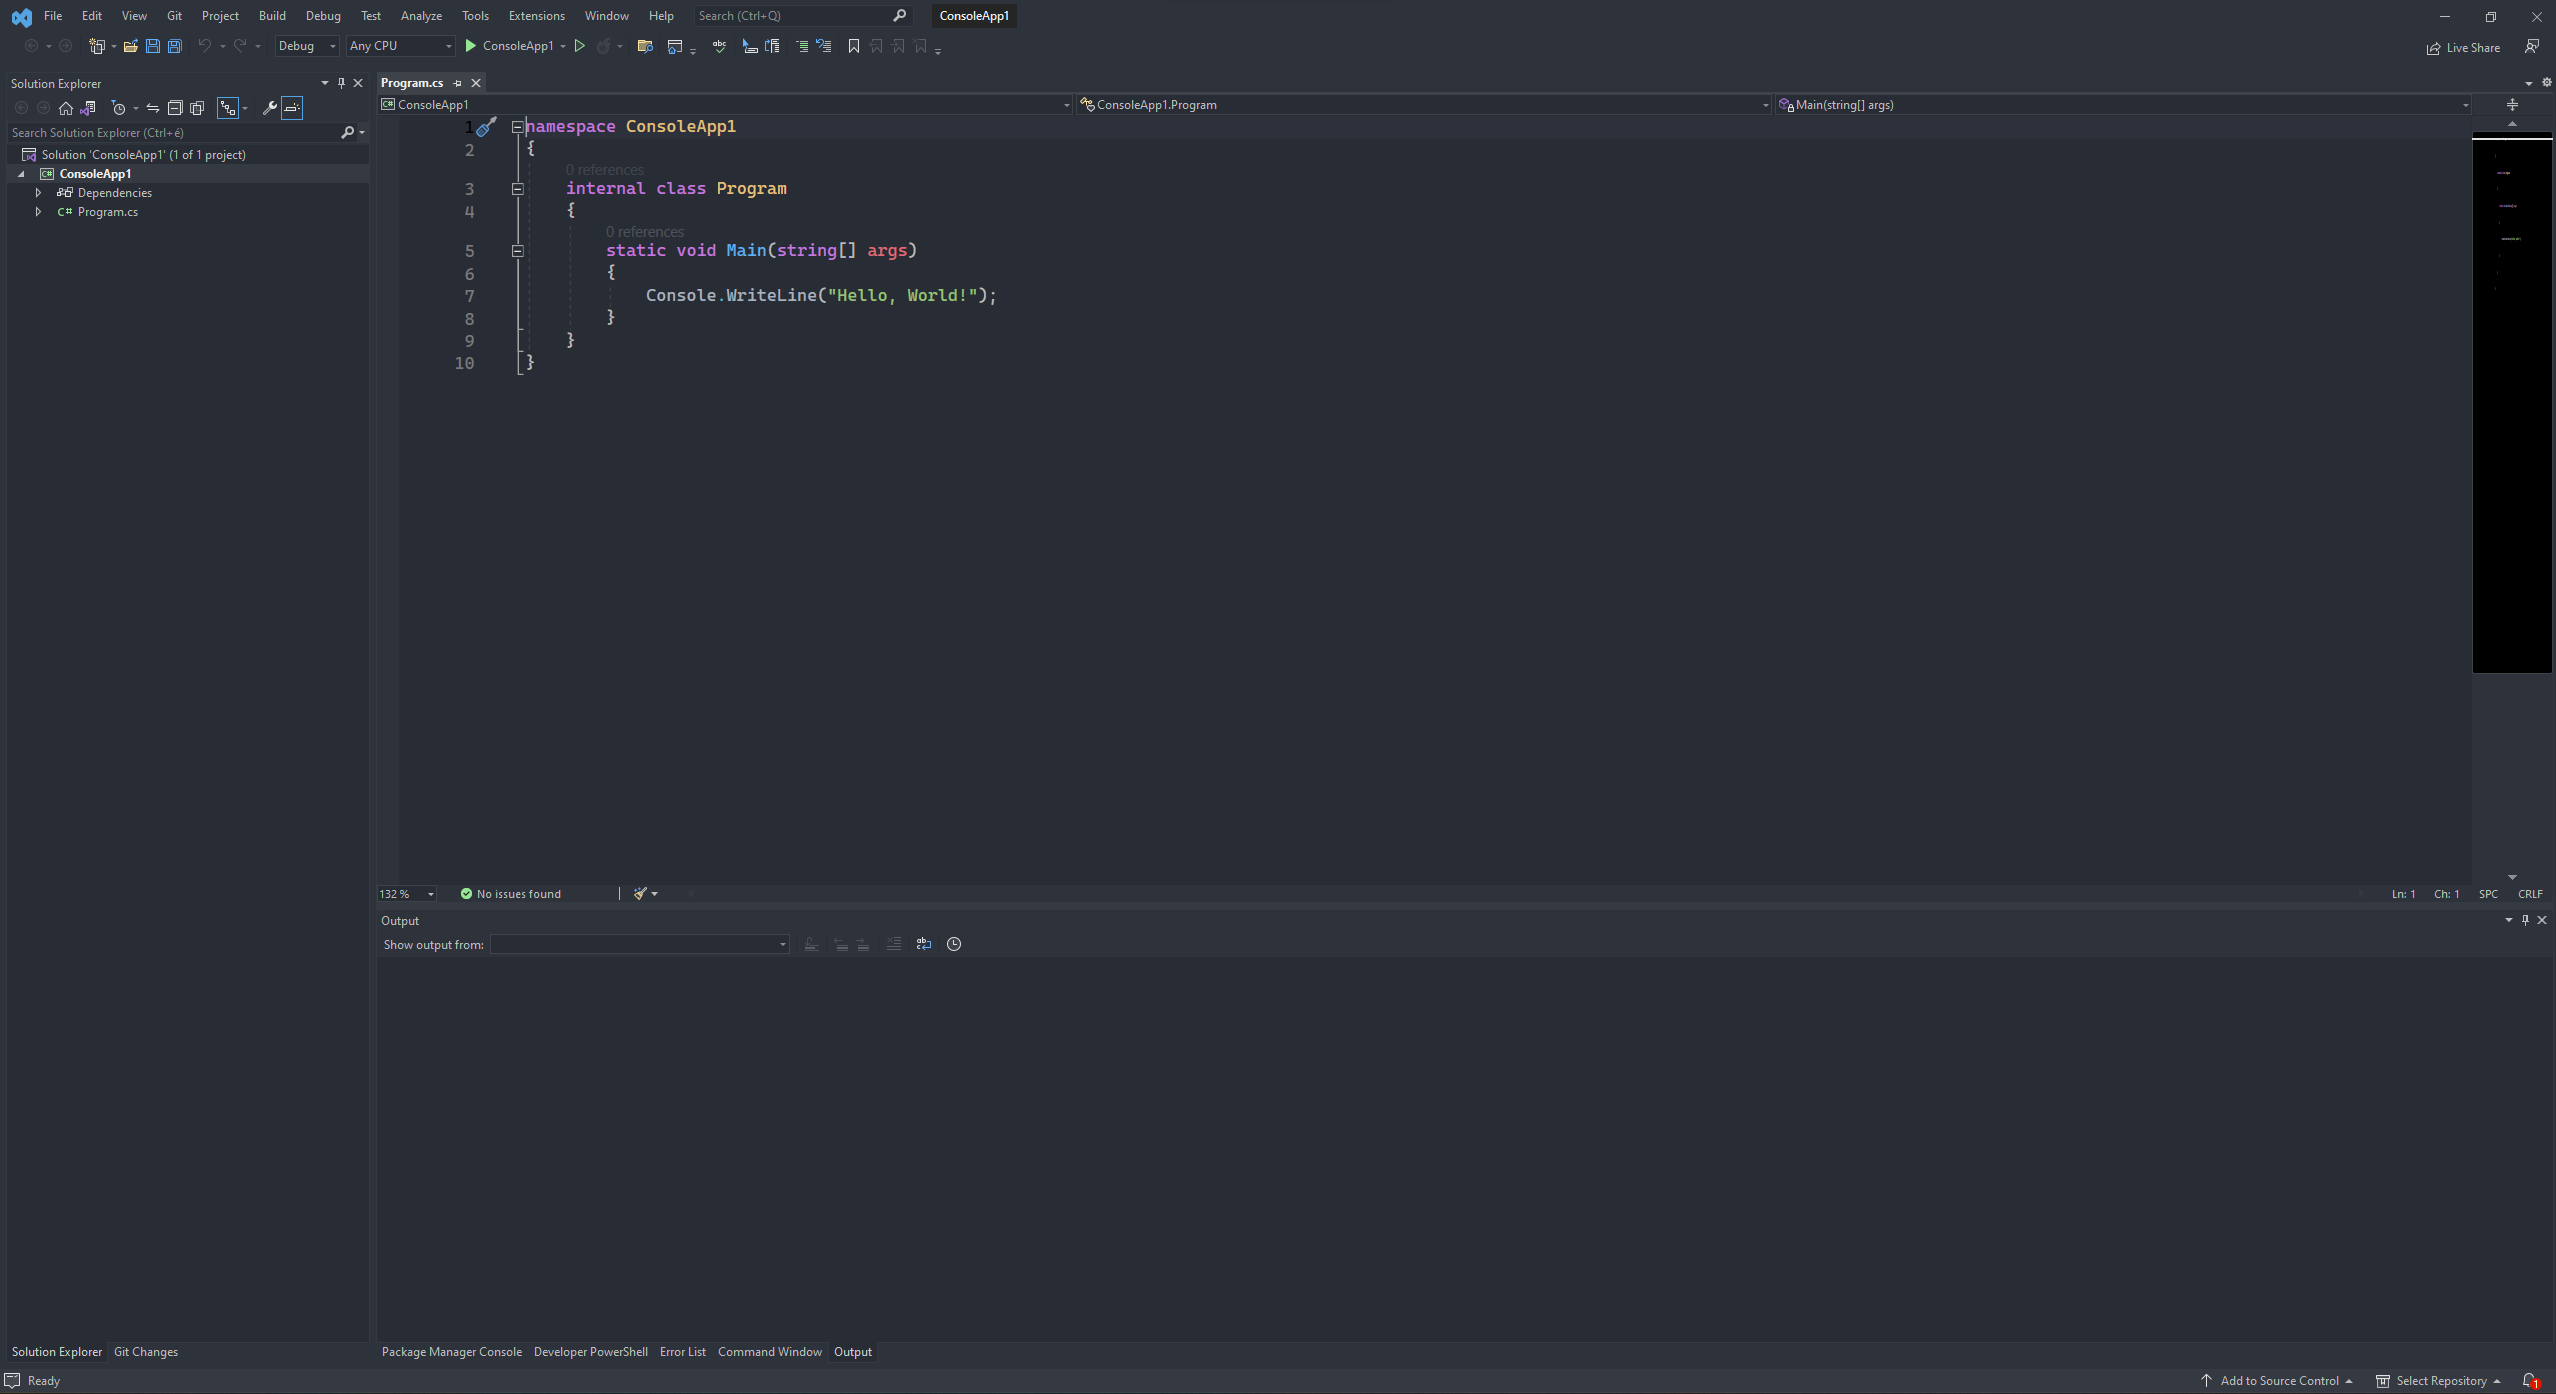
\includegraphics[width=12.0truecm]{images/VisualStuido2022.png}
    \caption{Visual Studio 2022}
    \label{fig:VisualStuido2022}
\end{figure}
Míg a Visual Studio elsősorban a Windows operációs rendszerre lett tervezve, a Microsoft kiadott egy könnyebb, keresztplatformos változatot is, a Visual Studio Code-ot. Ez utóbbi támogatja a Linux és macOS operációs rendszereket is, így a fejlesztők választhatnak az operációs rendszerüknek legmegfelelőbb változat közül.

Mindkét platform lehetővé teszi az együttműködést és a csapatmunkát, és számos bővítményt és sablont kínál a gyors és hatékony fejlesztés érdekében.